%Reneeth @BS17B025
%To create a pdf with the python environment

\documentclass{article}
\usepackage[utf8]{inputenc}
\usepackage[T1]{fontenc}
\usepackage[utf8]{inputenc}
\usepackage{lmodern}
\usepackage[a4paper, margin=1in]{geometry}

\usepackage{hyperref}
\hypersetup{
    colorlinks=true,
    linkcolor=black,
    filecolor=magenta,      
    urlcolor=green,
}

\usepackage[dvipsnames]{xcolor}
\definecolor{green}{RGB}{0,128,0}
\definecolor{teal}{RGB}{0,128,128}
\definecolor{limegreen}{RGB}{200, 130, 110}
\definecolor{cyan}{RGB}{150,200,210}


\renewcommand{\thesection}{\Roman{section}}


\usepackage{minted}
\large
\title{Programming Assignment 3}

%%%%%%%%%%%%%%%%%%%%%%%%%%%%%%%%%%%%%%%%%%%%%%%%%%%%%%%%%%%%%%%%%%%%%%%%%%%%%%%%%%%%%%%%%%%%%

\begin{document}
\begin{titlepage}
	\begin{center}
    \line(1,0){300}\\
    [0.65cm]
	\huge{\bfseries Programming Assignment III}\\
	\line(1,0){300}\\
	\textsc{\Large CS5691: Pattern Recognition and Machine Learning}\\
	\textsc{\large{Team 17 CCS Section Spring 2021}}\\
	\textsc{ \small{\today}}\\
	[5.5cm]     
	\end{center}
	\begin{flushright}
		\textsc{\Large Aanand Krishnan\\\small{BE17B001}}\\
		[0.5cm]
		\textsc{\Large Manoranjan J\\ \small{NA17B112}}\\
		[0.5cm]
		\textsc{\Large Reneeth Krishna MG\\\small{BS17B025}}
	\end{flushright}
\end{titlepage}
\tableofcontents
\newpage


\section{Pattern classification on linearly separable data}
\subsection{\textcolor{teal}{Python Code}}

\begin{minted}[frame=lines, linenos, fontsize=\large]
{python}

#1A part I perceptron

import pandas as pd
import numpy as np
from matplotlib import pyplot as plt
import matplotlib.cm as cm
import matplotlib.colors as colors
from tqdm import tqdm

class perceptron():
    def __init__(self,data1,data2):
        self.data1 = data1
        self.data2 = data2
        self.data = np.concatenate((data1,data2),axis=0)
        self.labels = [data1[0,-1],data2[0,-1]]
        self.weights = None
        self.error_epoch = None
    def train(self,eta,epochs):
        y1 = np.ones((len(self.data1),1))
        y2 = -1*np.ones((len(self.data2),1))
        data = self.data
        N,dim = data[:,:-1].shape
        X = np.concatenate((np.ones((N,1)),data[:,:-1]),axis=1)
        y = np.concatenate((y1,y2),axis=0)
        Xy = np.concatenate((X,np.reshape(y,(len(y),1))),axis=1)
        w = np.random.rand(1,1+dim)
        e = 1
        error_epoch = []
        
        pbar = tqdm(total=epochs,position=0,leave=True)
        while e<=epochs:
            e += 1
            pbar.update(1)
            np.random.shuffle(Xy)
            for i in range(N):
                w = w + ((eta/2)*(Xy[i,-1]-np.sign(Xy[i,:-1]@w.T))*Xy[i,:-1])
            error = 0
            for i in range(N):
                error += (1/2)*abs((Xy[i,-1]-np.sign(Xy[i,:-1]@w.T)))*
                (Xy[i,:-1]@w.T)*Xy[i,-1]
            error_epoch.append(-error)
        pbar.close()
        self.weights = w
        self.error_epoch = np.array(error_epoch)
        return None
    def classify(self,data):
        w = self.weights
        labels = self.labels
        l = [0]+labels 
        return np.array([l[int(i)] for i in np.sign(np.concatenate((np.ones(
        (len(data),1)),data),axis=1)@w.T)])
    def plot_error(self):
        plt.plot(self.error_epoch)
        return None

f = pd.read_csv('17/train.csv',header = None)
data_tr0 = (f[f[2]==0]).to_numpy()
data_tr1 = (f[f[2]==1]).to_numpy()
data_tr2 = (f[f[2]==2]).to_numpy()
data_tr3 = (f[f[2]==3]).to_numpy()
f = pd.read_csv('17/dev.csv',header = None)
data_te0 = (f[f[2]==0]).to_numpy()
data_te1 = (f[f[2]==1]).to_numpy()
data_te2 = (f[f[2]==2]).to_numpy()
data_te3 = (f[f[2]==3]).to_numpy()   

eta = 0.1
epochs = 10
#01
p01 = perceptron(data_tr0,data_tr1)
p01.train(eta,epochs)
data_tr01 = np.concatenate((data_tr0,data_tr1),axis=0)
train_acc_01 = 100*((data_tr01[:,-1]==p01.classify(data_tr01[:,:-1]))
                    .mean())
print('train_acc_01 = %f'%(train_acc_01))
data_te01 = np.concatenate((data_te0,data_te1),axis=0)
test_acc_01 = 100*((data_te01[:,-1]==p01.classify(data_te01[:,:-1]))
                  .mean())
print('test_acc_01 = %f'%(test_acc_01))

#02
p02 = perceptron(data_tr0,data_tr2)
p02.train(eta,epochs)
data_tr02 = np.concatenate((data_tr0,data_tr2),axis=0)
train_acc_02 = 100*((data_tr02[:,-1]==p02.classify(data_tr02[:,:-1]))
                    .mean())
print('train_acc_02 = %f'%(train_acc_02))
data_te02 = np.concatenate((data_te0,data_te2),axis=0)
test_acc_02 = 100*((data_te02[:,-1]==p02.classify(data_te02[:,:-1]))
                .mean())
print('test_acc_02 = %f'%(test_acc_02))

#03
p03 = perceptron(data_tr0,data_tr3)
p03.train(eta,epochs)
data_tr03 = np.concatenate((data_tr0,data_tr3),axis=0)
train_acc_03 = 100*((data_tr03[:,-1]==p03.classify(data_tr03[:,:-1]))
                   .mean())
print('train_acc_03 = %f'%(train_acc_03))
data_te03 = np.concatenate((data_te0,data_te3),axis=0)
test_acc_03 = 100*((data_te03[:,-1]==p03.classify(data_te03[:,:-1]))
                  .mean())
print('test_acc_03 = %f'%(test_acc_03))
#12
p12 = perceptron(data_tr1,data_tr2)
p12.train(eta,epochs)
data_tr12 = np.concatenate((data_tr1,data_tr2),axis=0)
train_acc_12 = 100*((data_tr12[:,-1]==p12.classify(data_tr12[:,:-1]))
                    .mean())
print('train_acc_12 = %f'%(train_acc_12))
data_te12 = np.concatenate((data_te1,data_te2),axis=0)
test_acc_12 = 100*((data_te12[:,-1]==p12.classify(data_te12[:,:-1]))
                  .mean())
print('test_acc_12 = %f'%(test_acc_12))
#13
p13 = perceptron(data_tr1,data_tr3)
p13.train(eta,epochs)
data_tr13 = np.concatenate((data_tr1,data_tr3),axis=0)
train_acc_13 = 100*((data_tr13[:,-1]==p13.classify(data_tr13[:,:-1]))
                   .mean())
print('train_acc_13 = %f'%(train_acc_13))
data_te13 = np.concatenate((data_te1,data_te3),axis=0)
test_acc_13 = 100*((data_te13[:,-1]==p13.classify(data_te13[:,:-1]))
                   .mean())
print('test_acc_13 = %f'%(test_acc_13))
#23
p23 = perceptron(data_tr2,data_tr3)
p23.train(eta,epochs)
data_tr23 = np.concatenate((data_tr2,data_tr3),axis=0)
train_acc_23 = 100*((data_tr23[:,-1]==p23.classify(data_tr23[:,:-1]))
                   .mean())
print('train_acc_23 = %f'%(train_acc_23))
data_te23 = np.concatenate((data_te2,data_te3),axis=0)
test_acc_23 = 100*((data_te23[:,-1]==p23.classify(data_te23[:,:-1]))
                  .mean())
print('test_acc_23 = %f'%(test_acc_23))

#plots
X_train = data_tr01
X_test = data_te01
# Decision Region Plots #####################################################
# define bounds of the domain
min1, max1 = X_train[:, 0].min()-1, X_train[:, 0].max()+1
min2, max2 = X_train[:, 1].min()-1, X_train[:, 1].max()+1

# define the x and y scale
x1_grid = np.arange(min1, max1, 0.1)
x2_grid = np.arange(min2, max2, 0.1)

x1_grid, x2_grid = np.meshgrid(x1_grid, x2_grid)

c1, c2 = x1_grid.flatten(), x1_grid.flatten()
c1, c2 = x1_grid.reshape((len(c1), 1)), x2_grid.reshape((len(c2), 1))

x = np.hstack((c1,c2))

y_pred = p01.classify(x)

x3_grid = y_pred.reshape(x1_grid.shape)



fig = plt.figure(1,figsize=(7.5,4))
ax = fig.add_subplot(111)
cmap =plt.get_cmap('Paired',2)
cs = ax.contourf(x1_grid, x2_grid, x3_grid, cmap=cmap)
ax.scatter(X_train[:,0],X_train[:,1],marker='x',
        color = 'blue',label='train data')
ax.scatter(X_test[:,0],X_test[:,1],marker='x',
        color='black',label='test data')
ax.legend()
ax.set_xlabel('x1',fontsize=10)
ax.set_ylabel('x2',fontsize=10)
ax.set_title('Perceptron : Labels (0,1)', fontsize=10)
cbar = plt.colorbar(cm.ScalarMappable(cmap=cmap),
                    ticks =[0.25,0.75])
cbar.ax.invert_yaxis()
cbar.set_ticklabels(['0','1'])

X_train = data_tr02
X_test = data_te02
# Decision Region Plots #####################################################
# define bounds of the domain
min1, max1 = X_train[:, 0].min()-1, X_train[:, 0].max()+1
min2, max2 = X_train[:, 1].min()-1, X_train[:, 1].max()+1

# define the x and y scale
x1_grid = np.arange(min1, max1, 0.1)
x2_grid = np.arange(min2, max2, 0.1)

x1_grid, x2_grid = np.meshgrid(x1_grid, x2_grid)

c1, c2 = x1_grid.flatten(), x1_grid.flatten()
c1, c2 = x1_grid.reshape((len(c1), 1)),
        x2_grid.reshape((len(c2), 1))

x = np.hstack((c1,c2))

y_pred = p02.classify(x)

x3_grid = y_pred.reshape(x1_grid.shape)



fig = plt.figure(2,figsize=(7.5,4))
ax = fig.add_subplot(111)
cmap =plt.get_cmap('Paired',2)
cs = ax.contourf(x1_grid, x2_grid, x3_grid, cmap=cmap)
ax.scatter(X_train[:,0],X_train[:,1],marker='x',
           color = 'blue',label='train data')
ax.scatter(X_test[:,0],X_test[:,1],marker='x',
             color='black',label='test data')
ax.legend()
ax.set_xlabel('x1',fontsize=10)
ax.set_ylabel('x2',fontsize=10)
ax.set_title('Perceptron : Labels (0,2)', fontsize=10)
cbar = plt.colorbar(cm.ScalarMappable(cmap=cmap),ticks =[0.25,0.75])
cbar.ax.invert_yaxis()
cbar.set_ticklabels(['0','2'])

X_train = data_tr03
X_test = data_te03
# Decision Region Plots #####################################################
# define bounds of the domain
min1, max1 = X_train[:, 0].min()-1, X_train[:, 0].max()+1
min2, max2 = X_train[:, 1].min()-1, X_train[:, 1].max()+1

# define the x and y scale
x1_grid = np.arange(min1, max1, 0.1)
x2_grid = np.arange(min2, max2, 0.1)

x1_grid, x2_grid = np.meshgrid(x1_grid, x2_grid)

c1, c2 = x1_grid.flatten(), x1_grid.flatten()
c1, c2 = x1_grid.reshape((len(c1), 1)),
            x2_grid.reshape((len(c2), 1))

x = np.hstack((c1,c2))

y_pred = p03.classify(x)

x3_grid = y_pred.reshape(x1_grid.shape)



fig = plt.figure(3,figsize=(7.5,4))
ax = fig.add_subplot(111)
cmap =plt.get_cmap('Paired',2)
cs = ax.contourf(x1_grid, x2_grid, x3_grid, cmap=cmap)
ax.scatter(X_train[:,0],X_train[:,1],marker='x',
            color = 'blue',label='train data')
ax.scatter(X_test[:,0],X_test[:,1],marker='x',
           color='black',label='test data')
ax.legend()
ax.set_xlabel('x1',fontsize=10)
ax.set_ylabel('x2',fontsize=10)
ax.set_title('Perceptron : Labels (0,3)', fontsize=10)
cbar = plt.colorbar(cm.ScalarMappable(cmap=cmap),
        ticks =[0.25,0.75])
cbar.ax.invert_yaxis()
cbar.set_ticklabels(['0','3'])

X_train = data_tr12
X_test = data_te12
# Decision Region Plots #####################################################
# define bounds of the domain
min1, max1 = X_train[:, 0].min()-1, X_train[:, 0].max()+1
min2, max2 = X_train[:, 1].min()-1, X_train[:, 1].max()+1

# define the x and y scale
x1_grid = np.arange(min1, max1, 0.1)
x2_grid = np.arange(min2, max2, 0.1)

x1_grid, x2_grid = np.meshgrid(x1_grid, x2_grid)

c1, c2 = x1_grid.flatten(), x1_grid.flatten()
c1, c2 = x1_grid.reshape((len(c1), 1)),
           x2_grid.reshape((len(c2), 1))

x = np.hstack((c1,c2))

y_pred = p12.classify(x)

x3_grid = y_pred.reshape(x1_grid.shape)



fig = plt.figure(4,figsize=(7.5,4))
ax = fig.add_subplot(111)
cmap =plt.get_cmap('Paired',2)
cs = ax.contourf(x1_grid, x2_grid, x3_grid, cmap=cmap)
ax.scatter(X_train[:,0],X_train[:,1],marker='x',
           color = 'blue',label='train data')
ax.scatter(X_test[:,0],X_test[:,1],marker='x',
            color='black',label='test data')
ax.legend()
ax.set_xlabel('x1',fontsize=10)
ax.set_ylabel('x2',fontsize=10)
ax.set_title('Perceptron : Labels (1,2)', fontsize=10)
cbar = plt.colorbar(cm.ScalarMappable(cmap=cmap),
                    ticks =[0.25,0.75])
cbar.ax.invert_yaxis()
cbar.set_ticklabels(['1','2'])

X_train = data_tr13
X_test = data_te13
# Decision Region Plots #####################################################
# define bounds of the domain
min1, max1 = X_train[:, 0].min()-1, X_train[:, 0].max()+1
min2, max2 = X_train[:, 1].min()-1, X_train[:, 1].max()+1

# define the x and y scale
x1_grid = np.arange(min1, max1, 0.1)
x2_grid = np.arange(min2, max2, 0.1)

x1_grid, x2_grid = np.meshgrid(x1_grid, x2_grid)

c1, c2 = x1_grid.flatten(), x1_grid.flatten()
c1, c2 = x1_grid.reshape((len(c1), 1)), 
                    x2_grid.reshape((len(c2), 1))

x = np.hstack((c1,c2))

y_pred = p13.classify(x)

x3_grid = y_pred.reshape(x1_grid.shape)



fig = plt.figure(5,figsize=(7.5,4))
ax = fig.add_subplot(111)
cmap =plt.get_cmap('Paired',2)
cs = ax.contourf(x1_grid, x2_grid, x3_grid, cmap=cmap)
ax.scatter(X_train[:,0],X_train[:,1],marker='x',
            color = 'blue',label='train data')
ax.scatter(X_test[:,0],X_test[:,1],marker='x', 
             color='black',label='test data')
ax.legend()
ax.set_xlabel('x1',fontsize=10)
ax.set_ylabel('x2',fontsize=10)
ax.set_title('Perceptron : Labels (1,3)', fontsize=10)
cbar = plt.colorbar(cm.ScalarMappable(cmap=cmap),
          ticks =[0.25,0.75])
cbar.ax.invert_yaxis()
cbar.set_ticklabels(['1','3'])

X_train = data_tr23
X_test = data_te23
# Decision Region Plots #####################################################
# define bounds of the domain
min1, max1 = X_train[:, 0].min()-1, X_train[:, 0].max()+1
min2, max2 = X_train[:, 1].min()-1, X_train[:, 1].max()+1

# define the x and y scale
x1_grid = np.arange(min1, max1, 0.1)
x2_grid = np.arange(min2, max2, 0.1)

x1_grid, x2_grid = np.meshgrid(x1_grid, x2_grid)

c1, c2 = x1_grid.flatten(), x1_grid.flatten()
c1, c2 = x1_grid.reshape((len(c1), 1)), 
          x2_grid.reshape((len(c2), 1))

x = np.hstack((c1,c2))

y_pred = p23.classify(x)

x3_grid = y_pred.reshape(x1_grid.shape)



fig = plt.figure(6,figsize=(7.5,4))
ax = fig.add_subplot(111)
cmap =plt.get_cmap('Paired',2)
cs = ax.contourf(x1_grid, x2_grid, x3_grid, cmap=cmap)
ax.scatter(X_train[:,0],X_train[:,1],marker='x',
               color = 'blue',label='train data')
ax.scatter(X_test[:,0],X_test[:,1],marker='x',
            color='black',label='test data')
ax.legend()
ax.set_xlabel('x1',fontsize=10)
ax.set_ylabel('x2',fontsize=10)
ax.set_title('Perceptron : Labels (2,3)', fontsize=10)
cbar = plt.colorbar(cm.ScalarMappable(cmap=cmap),
                ticks =[0.25,0.75])
cbar.ax.invert_yaxis()
cbar.set_ticklabels(['2','3'])

#1A part II MLFNN

from sklearn import preprocessing
import pandas as pd
import numpy as np
import torch as tc
from matplotlib import pyplot as plt
import matplotlib.cm as cm
import matplotlib.colors as colors
from tqdm import tqdm

f = pd.read_csv('17/train.csv',header = None)
data_tr = f.to_numpy()
f = pd.read_csv('17/dev.csv',header = None)
data_te = f.to_numpy()
#1 to K categorial 1 hot vector transformation
labelenc = preprocessing.LabelBinarizer()  
Xtr = (tc.from_numpy(data_tr[:,:-1])).float()
ytr = (tc.from_numpy(labelenc.fit_transform(data_tr[:,-1])))
                    .float()
Xte = (tc.from_numpy(data_te[:,:-1])).float()
yte = (tc.from_numpy(labelenc.fit_transform(data_te[:,-1])))
                    .float()

epochs = 10000

inp_l = 2
hid_l = 4
out_l = 4
#activation fxns : Sigmoid,Tanh,SOftmax,ReLU,ELU,SELU,CELU,
mlfnn = tc.nn.Sequential(tc.nn.Linear(inp_l,hid_l),
                         tc.nn.ELU(),tc.nn.Linear(hid_l,out_l))
MSE = tc.nn.MSELoss()
optimizer = tc.optim.SGD(mlfnn.parameters(), lr=0.001)
from tqdm import tqdm
epochs = 10000
pbar = tqdm(total=epochs,position=0,leave=True)
for i in range(epochs):
    
    optimizer.zero_grad() 
    ytrp = mlfnn(Xtr)
    loss = MSE(ytrp,ytr)
    loss.backward()
    optimizer.step()
    pbar.update(1)
pbar.close()
tr_acc = 100*((data_tr[:,-1] == labelenc.
                    inverse_transform(mlfnn(Xtr))).mean())
te_acc = 100*((data_te[:,-1] == labelenc.
                     inverse_transform(mlfnn(Xte))).mean())
print('train acc = %f'%(tr_acc))
print('test acc = %f'%(te_acc))

#plotting
X_train = data_tr[:,:-1]
X_test = data_te[:,:-1]
# Decision Region Plots #####################################################
# define bounds of the domain
min1, max1 = X_train[:, 0].min()-1, X_train[:, 0].max()+1
min2, max2 = X_train[:, 1].min()-1, X_train[:, 1].max()+1

# define the x and y scale
x1_grid = np.arange(min1, max1, 0.1)
x2_grid = np.arange(min2, max2, 0.1)

x1_grid, x2_grid = np.meshgrid(x1_grid, x2_grid)

c1, c2 = x1_grid.flatten(), x1_grid.flatten()
c1, c2 = x1_grid.reshape((len(c1), 1)), x2_grid.
                           reshape((len(c2), 1))

x = np.hstack((c1,c2))

y_pred = labelenc.inverse_transform(mlfnn(tc.from_numpy(x)
                                    .float()))

x3_grid = y_pred.reshape(x1_grid.shape)


fig = plt.figure(1,figsize=(7.5,4))
ax = fig.add_subplot(111)
cmap =plt.get_cmap('Paired',4)
cs = ax.contourf(x1_grid, x2_grid, x3_grid, cmap=cmap)
ax.scatter(X_train[:,0],X_train[:,1],marker='x',
                color = 'blue',label='train data')
ax.scatter(X_test[:,0],X_test[:,1],marker='x',
                  color='black',label='test data')
ax.legend()
ax.set_xlabel('x1',fontsize=10)
ax.set_ylabel('x2',fontsize=10)
ax.set_title('MLFNN : All Four Labels', fontsize=10)
cbar = plt.colorbar(cm.ScalarMappable(cmap=cmap),
                  ticks=np.linspace(0.125,1-0.125,4))
cbar.ax.invert_yaxis()
cbar.set_ticklabels(['0','1','2','3'])

#1A part III linear svm
import numpy as np
import pandas as pd
from sklearn.svm import SVC
from matplotlib import pyplot as plt
import matplotlib.cm as cm
import matplotlib.colors as colors
from tqdm import tqdm

f = pd.read_csv('17/train.csv',header = None)
data_tr0 = (f[f[2]==0]).to_numpy()
data_tr1 = (f[f[2]==1]).to_numpy()
data_tr2 = (f[f[2]==2]).to_numpy()
data_tr3 = (f[f[2]==3]).to_numpy()
f = pd.read_csv('17/dev.csv',header = None)
data_te0 = (f[f[2]==0]).to_numpy()
data_te1 = (f[f[2]==1]).to_numpy()
data_te2 = (f[f[2]==2]).to_numpy()
data_te3 = (f[f[2]==3]).to_numpy()

#01
data_tr01 = np.concatenate((data_tr0,data_tr1),axis=0)
data_te01 = np.concatenate((data_te0,data_te1),axis=0)
svc01 = SVC(kernel='linear')
svc01.fit(data_tr01[:,:-1],data_tr01[:,-1])
train_acc_01 = 100*((data_tr01[:,-1]==svc01.
                    predict(data_tr01[:,:-1])).mean())
print('train_acc_01 = %f'%(train_acc_01))
test_acc_01 = 100*((data_te01[:,-1]==svc01.
                    predict(data_te01[:,:-1])).mean())
print('test_acc_01 = %f'%(test_acc_01))

#02
data_tr02 = np.concatenate((data_tr0,data_tr2),axis=0)
data_te02 = np.concatenate((data_te0,data_te2),axis=0)
svc02 = SVC(kernel='linear')
svc02.fit(data_tr02[:,:-1],data_tr02[:,-1])
train_acc_02 = 100*((data_tr02[:,-1]==svc02.
                    predict(data_tr02[:,:-1])).mean())
print('train_acc_02 = %f'%(train_acc_02))
test_acc_02 = 100*((data_te02[:,-1]==svc02.
                    predict(data_te02[:,:-1])).mean())
print('test_acc_02 = %f'%(test_acc_02))

#03
data_tr03 = np.concatenate((data_tr0,data_tr3),axis=0)
data_te03 = np.concatenate((data_te0,data_te3),axis=0)
svc03 = SVC(kernel='linear')
svc03.fit(data_tr03[:,:-1],data_tr03[:,-1])
train_acc_03 = 100*((data_tr03[:,-1]==svc03.
                    predict(data_tr03[:,:-1])).mean())
print('train_acc_03 = %f'%(train_acc_03))
test_acc_03 = 100*((data_te03[:,-1]==svc03.
                     predict(data_te03[:,:-1])).mean())
print('test_acc_03 = %f'%(test_acc_03))

#12
data_tr12 = np.concatenate((data_tr1,data_tr2),axis=0)
data_te12 = np.concatenate((data_te1,data_te2),axis=0)
svc12 = SVC(kernel='linear')
svc12.fit(data_tr12[:,:-1],data_tr12[:,-1])
train_acc_12 = 100*((data_tr12[:,-1]==svc12.
                      predict(data_tr12[:,:-1])).mean())
print('train_acc_12 = %f'%(train_acc_12))
test_acc_12 = 100*((data_te12[:,-1]==svc12.
                       predict(data_te12[:,:-1])).mean())
print('test_acc_12 = %f'%(test_acc_12))

#13
data_tr13 = np.concatenate((data_tr1,data_tr3),axis=0)
data_te13 = np.concatenate((data_te1,data_te3),axis=0)
svc13 = SVC(kernel='linear')
svc13.fit(data_tr13[:,:-1],data_tr13[:,-1])
train_acc_13 = 100*((data_tr13[:,-1]==svc13.
                       predict(data_tr13[:,:-1])).mean())
print('train_acc_13 = %f'%(train_acc_13))
test_acc_13 = 100*((data_te13[:,-1]==svc13.
                       predict(data_te13[:,:-1])).mean())
print('test_acc_13 = %f'%(test_acc_13))

#23
data_tr23 = np.concatenate((data_tr2,data_tr3),axis=0)
data_te23 = np.concatenate((data_te2,data_te3),axis=0)
svc23 = SVC(kernel='linear')
svc23.fit(data_tr23[:,:-1],data_tr23[:,-1])
train_acc_23 = 100*((data_tr23[:,-1]==svc23.
                      predict(data_tr23[:,:-1])).mean())
print('train_acc_23 = %f'%(train_acc_23))
test_acc_23 = 100*((data_te23[:,-1]==svc23.
                      predict(data_te23[:,:-1])).mean())
print('test_acc_23 = %f'%(test_acc_23))

#plots
X_train = data_tr01
X_test = data_te01
# Decision Region Plots #####################################################
# define bounds of the domain
min1, max1 = X_train[:, 0].min()-1, X_train[:, 0].max()+1
min2, max2 = X_train[:, 1].min()-1, X_train[:, 1].max()+1

# define the x and y scale
x1_grid = np.arange(min1, max1, 0.1)
x2_grid = np.arange(min2, max2, 0.1)

x1_grid, x2_grid = np.meshgrid(x1_grid, x2_grid)

c1, c2 = x1_grid.flatten(), x1_grid.flatten()
c1, c2 = x1_grid.reshape((len(c1), 1)), x2_grid.
                         reshape((len(c2), 1))

x = np.hstack((c1,c2))

y_pred = svc01.predict(x)

x3_grid = y_pred.reshape(x1_grid.shape)

suppvec = svc01.support_vectors_

fig = plt.figure(1,figsize=(7.5,4))
ax = fig.add_subplot(111)
cmap =plt.get_cmap('Paired',2)
cs = ax.contourf(x1_grid, x2_grid, x3_grid, cmap=cmap)
ax.scatter(X_train[:,0],X_train[:,1],marker='x',
                     color = 'blue',label='train data')
ax.scatter(suppvec[:,0],suppvec[:,1],marker='x',
                  color='yellow',label='support vector')
ax.scatter(X_test[:,0],X_test[:,1],marker='x',
                         color='black',label='test data')
ax.legend()
ax.set_xlabel('x1',fontsize=10)
ax.set_ylabel('x2',fontsize=10)
ax.set_title('SVM : Labels (0,1)', fontsize=10)
cbar = plt.colorbar(cm.ScalarMappable(cmap=cmap),
                             ticks =[0.25,0.75])
cbar.ax.invert_yaxis()
cbar.set_ticklabels(['0','1'])



X_train = data_tr02
X_test = data_te02
# Decision Region Plots #####################################################
# define bounds of the domain
min1, max1 = X_train[:, 0].min()-1, X_train[:, 0].max()+1
min2, max2 = X_train[:, 1].min()-1, X_train[:, 1].max()+1

# define the x and y scale
x1_grid = np.arange(min1, max1, 0.1)
x2_grid = np.arange(min2, max2, 0.1)

x1_grid, x2_grid = np.meshgrid(x1_grid, x2_grid)

c1, c2 = x1_grid.flatten(), x1_grid.flatten()
c1, c2 = x1_grid.reshape((len(c1), 1)), 
             x2_grid.reshape((len(c2), 1))

x = np.hstack((c1,c2))

y_pred = svc02.predict(x)

x3_grid = y_pred.reshape(x1_grid.shape)

suppvec = svc02.support_vectors_

fig = plt.figure(2,figsize=(7.5,4))
ax = fig.add_subplot(111)
cmap =plt.get_cmap('Paired',2)
cs = ax.contourf(x1_grid, x2_grid, x3_grid, cmap=cmap)
ax.scatter(X_train[:,0],X_train[:,1],marker='x',
             color = 'blue',label='train data')
ax.scatter(suppvec[:,0],suppvec[:,1],marker='x',
            color='yellow',label='support vector')
ax.scatter(X_test[:,0],X_test[:,1],marker='x',
                  color='black',label='test data')
ax.legend()
ax.set_xlabel('x1',fontsize=10)
ax.set_ylabel('x2',fontsize=10)
ax.set_title('SVM : Labels (0,2)', fontsize=10)
cbar = plt.colorbar(cm.ScalarMappable(cmap=cmap),
                            ticks =[0.25,0.75])
cbar.ax.invert_yaxis()
cbar.set_ticklabels(['0','2'])

X_train = data_tr03
X_test = data_te03
# Decision Region Plots #####################################################
# define bounds of the domain
min1, max1 = X_train[:, 0].min()-1, X_train[:, 0].max()+1
min2, max2 = X_train[:, 1].min()-1, X_train[:, 1].max()+1

# define the x and y scale
x1_grid = np.arange(min1, max1, 0.1)
x2_grid = np.arange(min2, max2, 0.1)

x1_grid, x2_grid = np.meshgrid(x1_grid, x2_grid)

c1, c2 = x1_grid.flatten(), x1_grid.flatten()
c1, c2 = x1_grid.reshape((len(c1), 1)), x2_grid.
                            reshape((len(c2), 1))

x = np.hstack((c1,c2))

y_pred = svc03.predict(x)

x3_grid = y_pred.reshape(x1_grid.shape)

suppvec = svc03.support_vectors_

fig = plt.figure(3,figsize=(7.5,4))
ax = fig.add_subplot(111)
cmap =plt.get_cmap('Paired',2)
cs = ax.contourf(x1_grid, x2_grid, x3_grid, cmap=cmap)
ax.scatter(X_train[:,0],X_train[:,1],marker='x',
                color = 'blue',label='train data')
ax.scatter(suppvec[:,0],suppvec[:,1],marker='x',
            color='yellow',label='support vector')
ax.scatter(X_test[:,0],X_test[:,1],marker='x',
                  color='black',label='test data')
ax.legend()
ax.set_xlabel('x1',fontsize=10)
ax.set_ylabel('x2',fontsize=10)
ax.set_title('SVM : Labels (0,3)', fontsize=10)
cbar = plt.colorbar(cm.ScalarMappable(cmap=cmap),
                             ticks =[0.25,0.75])
cbar.ax.invert_yaxis()
cbar.set_ticklabels(['0','3'])

X_train = data_tr12
X_test = data_te12
# Decision Region Plots #####################################################
# define bounds of the domain
min1, max1 = X_train[:, 0].min()-1, X_train[:, 0].max()+1
min2, max2 = X_train[:, 1].min()-1, X_train[:, 1].max()+1

# define the x and y scale
x1_grid = np.arange(min1, max1, 0.1)
x2_grid = np.arange(min2, max2, 0.1)

x1_grid, x2_grid = np.meshgrid(x1_grid, x2_grid)

c1, c2 = x1_grid.flatten(), x1_grid.flatten()
c1, c2 = x1_grid.reshape((len(c1), 1)), x2_grid.
                           reshape((len(c2), 1))

x = np.hstack((c1,c2))

y_pred = svc12.predict(x)

x3_grid = y_pred.reshape(x1_grid.shape)

suppvec = svc12.support_vectors_

fig = plt.figure(4,figsize=(7.5,4))
ax = fig.add_subplot(111)
cmap =plt.get_cmap('Paired',2)
cs = ax.contourf(x1_grid, x2_grid, x3_grid, cmap=cmap)
ax.scatter(X_train[:,0],X_train[:,1],marker='x',
               color = 'blue',label='train data')
ax.scatter(suppvec[:,0],suppvec[:,1],marker='x',
             color='yellow',label='support vector')
ax.scatter(X_test[:,0],X_test[:,1],marker='x',
                  color='black',label='test data')
ax.legend()
ax.set_xlabel('x1',fontsize=10)
ax.set_ylabel('x2',fontsize=10)
ax.set_title('SVM : Labels (1,2)', fontsize=10)
cbar = plt.colorbar(cm.ScalarMappable(cmap=cmap),
                             ticks =[0.25,0.75])
cbar.ax.invert_yaxis()
cbar.set_ticklabels(['1','2'])

X_train = data_tr13
X_test = data_te13
# Decision Region Plots #####################################################
# define bounds of the domain
min1, max1 = X_train[:, 0].min()-1, X_train[:, 0].max()+1
min2, max2 = X_train[:, 1].min()-1, X_train[:, 1].max()+1

# define the x and y scale
x1_grid = np.arange(min1, max1, 0.1)
x2_grid = np.arange(min2, max2, 0.1)

x1_grid, x2_grid = np.meshgrid(x1_grid, x2_grid)

c1, c2 = x1_grid.flatten(), x1_grid.flatten()
c1, c2 = x1_grid.reshape((len(c1), 1)), x2_grid.
                           reshape((len(c2), 1))

x = np.hstack((c1,c2))

y_pred = svc13.predict(x)

x3_grid = y_pred.reshape(x1_grid.shape)

suppvec = svc13.support_vectors_

fig = plt.figure(5,figsize=(7.5,4))
ax = fig.add_subplot(111)
cmap =plt.get_cmap('Paired',2)
cs = ax.contourf(x1_grid, x2_grid, x3_grid, cmap=cmap)
ax.scatter(X_train[:,0],X_train[:,1],marker='x',
                       color = 'blue',label='train data')
ax.scatter(suppvec[:,0],suppvec[:,1],marker='x',
                   color='yellow',label='support vector')
ax.scatter(X_test[:,0],X_test[:,1],marker='x',
                        color='black',label='test data')
ax.legend()
ax.set_xlabel('x1',fontsize=10)
ax.set_ylabel('x2',fontsize=10)
ax.set_title('SVM : Labels (1,3)', fontsize=10)
cbar = plt.colorbar(cm.ScalarMappable(cmap=cmap),ticks =[0.25,0.75])
cbar.ax.invert_yaxis()
cbar.set_ticklabels(['1','3'])

X_train = data_tr23
X_test = data_te23
# Decision Region Plots #####################################################
# define bounds of the domain
min1, max1 = X_train[:, 0].min()-1, X_train[:, 0].max()+1
min2, max2 = X_train[:, 1].min()-1, X_train[:, 1].max()+1

# define the x and y scale
x1_grid = np.arange(min1, max1, 0.1)
x2_grid = np.arange(min2, max2, 0.1)

x1_grid, x2_grid = np.meshgrid(x1_grid, x2_grid)

c1, c2 = x1_grid.flatten(), x1_grid.flatten()
c1, c2 = x1_grid.reshape((len(c1), 1)), x2_grid.
                           reshape((len(c2), 1))

x = np.hstack((c1,c2))

y_pred = svc23.predict(x)

x3_grid = y_pred.reshape(x1_grid.shape)

suppvec = svc23.support_vectors_

fig = plt.figure(6,figsize=(7.5,4))
ax = fig.add_subplot(111)
cmap =plt.get_cmap('Paired',2)
cs = ax.contourf(x1_grid, x2_grid, x3_grid, cmap=cmap)
ax.scatter(X_train[:,0],X_train[:,1],marker='x',
                color = 'blue',label='train data')
ax.scatter(suppvec[:,0],suppvec[:,1],marker='x',
            color='yellow',label='support vector')
ax.scatter(X_test[:,0],X_test[:,1],marker='x',
                  color='black',label='test data')
ax.legend()
ax.set_xlabel('x1',fontsize=10)
ax.set_ylabel('x2',fontsize=10)
ax.set_title('SVM : Labels (2,3)', fontsize=10)
cbar = plt.colorbar(cm.ScalarMappable(cmap=cmap),
                             ticks =[0.25,0.75])
cbar.ax.invert_yaxis()
cbar.set_ticklabels(['2','3'])


\end{minted}

\newpage

\section{Pattern classification on non-linearly separable data}
\subsection{K nearest Neighbours Method and Bayes classifier with KNN for density estimation}
\subsubsection{\textcolor{teal}{Python Code}}

\begin{minted}[frame=lines, linenos, fontsize=\large]
{python}

# In[1]:
# Import Relevant Libraries
import numpy as np
import pandas as pd
import matplotlib.pyplot as plt
from sklearn.metrics import confusion_matrix
from mlxtend.plotting import plot_confusion_matrix
from sklearn.metrics import accuracy_score

import torch
from tqdm import tqdm

import torch.nn as nn
import torch.nn.functional as F
import torch.optim as optim
from functools import partial

#############################################################################

# In[2]:
# Read Data
# train data
train_data = pd.read_csv("datasets/Dataset_1b/train.csv",header=None)
    
# shuffle dataset
train_data = train_data.sample(frac=1)

# get train data
train_data = np.array(train_data)

# test data
test_data = pd.read_csv("datasets/Dataset_1b/dev.csv",header=None)

# shuffle dataset
test_data = test_data.sample(frac=1)

# get test data
test_data = np.array(test_data)

##############################################################################

# In[3]:
# Split training data
# length of data for fit
train_len = int(np.shape(train_data)[0])
val_len = int(np.shape(test_data)[0]*0.5)
test_len = int(np.shape(test_data)[0]*0.5)

X_train = train_data[:,0:2]
X_val = test_data[0:val_len,0:2]
X_test = test_data[val_len:val_len+test_len,0:2]

y_train = train_data[:,2]
y_val = test_data[0:val_len,2]
y_test = test_data[val_len:val_len+test_len,2]

##############################################################################

# In[4]:

# Build MLFFNN with 2 hidden layers using pytorch

class Net(nn.Module):
    def __init__(self):
        super(Net, self).__init__()
        
        # in_features = input dimension out_features -> to be tuned
        self.fc1 = nn.Linear(in_features=2, out_features=4)  
        
        # out_features -> to be tuned 
        self.fc2 = nn.Linear(in_features=4, out_features=4)
        
        # out_features = number of classes to be predicted
        self.fc3 = nn.Linear(in_features=4, out_features=3)
        
    def forward(self, x):
        x = F.relu(self.fc1(x))
        out1 = x
        x = F.relu(self.fc2(x))
        out2 = x
        x = self.fc3(x)
        return x,out1,out2

# In[5]:
    
# Initialize neural network class
net = Net()

# # transfer the model to GPU if available
# if torch.cuda.is_available():
#     print("using GPU")
#     net = net.cuda()
    
# In[6]:

########################################################################
# Define a Loss function and optimizer

# Both variables are to be tuned
num_epochs = 500        # desired number of training epochs.
learning_rate = 0.001

# loss function and optimizers can be changed
criterion = nn.CrossEntropyLoss()
optimizer = optim.Adam(net.parameters(), lr=learning_rate,weight_decay=5e-4)

num_params = np.sum([p.nelement() for p in net.parameters()])
print(num_params, ' parameters')

# In[7]:
# create dataloader for loading data

class myDataset(torch.utils.data.Dataset):
  
  #'Characterizes a dataset for PyTorch'
  def __init__(self,X,y,total_samples):
        #'Initialization'
        self.X = X
        self.y = y
        self.total_samples = total_samples
  
  def __len__(self):
        #'Denotes the total number of samples'
        return self.total_samples

  def __getitem__(self, index):
        #'Generates one sample of data'
        # Select sample
        # Load data and get label
        
        x_data = self.X[index,:]
        y_data = self.y[index]
        
        return x_data,y_data

# batch size can be changed to make epochs faster
params = {'batch_size': 16,
          'shuffle': False,
          'num_workers': 0}

# training dataset
training_set = myDataset(X_train,y_train,train_len)

training_generator = torch.utils.data.DataLoader(training_set, **params)

# validation dataset
validation_set = myDataset(X_val,y_val,val_len)
validation_generator = torch.utils.data.DataLoader(validation_set, **params)

# test dataset
test_set = myDataset(X_test,y_test,test_len)

test_generator = torch.utils.data.DataLoader(test_set, **params)

# In[8]:
    
def validation(model, loader):
    total_loss = 0
    accuracy = []
    tq = partial(tqdm, position=0, leave=True)
    
    model.eval()
    with torch.no_grad():
        for X, y in tq(loader):
          X = X.float()
          y = y.long()
          
          # if torch.cuda.is_available():
          #   X = X.cuda()
          #   y = y.cuda()
        
          prediction,_,_ = model(X)
          
          loss = criterion(prediction, y)
          
          prediction = F.softmax(prediction)
          
          acc = np.mean(np.array((torch.argmax(prediction,1) == y)))*100
          
          
          total_loss += loss.item()
          accuracy.append(acc)

    # print('Validation Accuracy: ', np.mean(np.array(accuracy)))   
    return total_loss/len(loader),np.mean(np.array(accuracy))


# In[9]:
    
def test(model, loader):
    y_pred = []
    accuracy = []
    tq = partial(tqdm, position=0, leave=True)
    
    model.eval()
    with torch.no_grad():
        for X, y in tq(loader):
          X = X.float()
          y = y.long()
          
          # if torch.cuda.is_available():
          #   X = X.cuda()
          #   y = y.cuda()
        
          prediction,_,_ = model(X)
          
          prediction = F.softmax(prediction)
          
          acc = np.mean(np.array((torch.argmax(prediction,1) == y)))*100

          accuracy.append(acc)

          prediction = torch.argmax(prediction,1)
          y_pred = y_pred + list(np.array(prediction))

    print('Test Accuracy: ', np.mean(np.array(accuracy)))   
    return y_pred,np.mean(np.array(accuracy))

# In[]:
    
def surface_plot(x1_grid,x2_grid,out1,out2,out3):
    
    for i in range(0,4):
        x3_grid = out1[:,i].detach().numpy()
        x3_grid = x3_grid.reshape(np.shape(x1_grid))
        
        fig = plt.figure(figsize=(16,12))
        ax = fig.add_subplot(111,projection='3d')
        ax.plot_surface(x1_grid,x2_grid,x3_grid,cmap='rainbow')
        ax.set_xlabel('X-axis(x1)',fontsize = 15) 
        ax.set_ylabel('Y-axis(x2)',fontsize = 15) 
        ax.set_zlabel('Z-axis(Node Output)',fontsize = 15)
        ax.set_title('Hidden Layer 1: Node' + str(i+1), fontsize=20)
        
        x3_grid = out2[:,i].detach().numpy()
        x3_grid = x3_grid.reshape(np.shape(x1_grid))
        
        fig = plt.figure(figsize=(16,12))
        ax = fig.add_subplot(111,projection='3d')
        ax.plot_surface(x1_grid,x2_grid,x3_grid,cmap='rainbow')
        ax.set_xlabel('X-axis(x1)',fontsize = 15) 
        ax.set_ylabel('Y-axis(x2)',fontsize = 15) 
        ax.set_zlabel('Z-axis(Node Output)',fontsize = 15)
        ax.set_title('Hidden Layer 2: Node' + str(i+1), fontsize=20)
        
    for i in range(0,3):
        x3_grid = out3[:,i].detach().numpy()
        x3_grid = x3_grid.reshape(np.shape(x1_grid))
        
        fig = plt.figure(figsize=(16,12))
        ax = fig.add_subplot(111,projection='3d')
        ax.plot_surface(x1_grid,x2_grid,x3_grid,cmap='rainbow')
        ax.set_xlabel('X-axis(x1)',fontsize = 15) 
        ax.set_ylabel('Y-axis(x2)',fontsize = 15) 
        ax.set_zlabel('Z-axis(Node Output)',fontsize = 15)
        ax.set_title('Output Layer: Node' + str(i+1), fontsize=20)
        
    
    

# In[10]:
    
tq = partial(tqdm, position=0, leave=True)

print('Start Training')
train_loss_list = []
train_accuracy_list = []

validation_loss_list = []
validation_accuracy_list = []

for epoch in range(0,num_epochs):
  print('epoch ', epoch + 1)
  loss = 0
  train_accuracy = []
  
  for X,y in tq(training_generator):
    
    X = X.float()
    y = y.long()
    # y = torch.squeeze(y,1)
    
    # if torch.cuda.is_available():
    #     X = X.cuda()
    #     y = y.cuda()
    
    
    optimizer.zero_grad()
    
    output,out1,out2 = net(X)
    loss = criterion(output,y)
    
    loss.backward()
    optimizer.step()

    loss += loss.item()
    
    prediction = F.softmax(output)
    
    accuracy = np.mean(np.array((torch.argmax(prediction,1) == y)))*100
    train_accuracy.append(accuracy) 

 
  
  train_loss_list.append([loss/len(training_generator)])
  # print(loss/len(training_generator))
  
  train_accuracy_list.append(np.mean(np.array(train_accuracy)))
  
  val_loss,val_accuracy = validation(net, validation_generator)

  validation_loss_list.append(val_loss)
  validation_accuracy_list.append(val_accuracy)
  
  if epoch == 0 or epoch == 4 or epoch == 19 or epoch == 99 
  or epoch == num_epochs-1:
      torch.save(net.state_dict(), 'models/model-'+str(epoch)+'.pth')
 
      
print(train_accuracy_list[-1])
print(validation_accuracy_list[-1])
  
# In[]:
net = Net()

# Import saved Model
net.load_state_dict(torch.load('models/model-499.pth'))
net.eval()
  
# In[11]:
    
# plt.plot(train_loss_list,label='Training Loss')
plt.plot(validation_loss_list,label='Validation Loss')
plt.xlabel('Number of Epochs')
plt.ylabel('Loss')
plt.title('Loss curve')
plt.legend()
plt.plot()

# In[12]:
    
plt.plot(train_accuracy_list,label='Training Accuracy')
plt.plot(validation_accuracy_list,label='Validation Accuracy')
plt.xlabel('Number of Epochs')
plt.ylabel('Accuracy')
plt.title('Accuracy curve')
plt.legend()
plt.show()

# In[13]:
    
y_pred, test_accuracy = test(net,test_generator)
print(test_accuracy)
c_matrix  = confusion_matrix(y_test, y_pred)

afig, ax = plot_confusion_matrix(conf_mat=c_matrix,figsize=(7,7),cmap=plt.cm.RdBu)
ax.set(title = "Confusion Matrix for test data")


y_pred, train_accuracy = test(net,training_generator)

c_matrix  = confusion_matrix(y_train, y_pred)

afig, ax = plot_confusion_matrix(conf_mat=c_matrix,figsize=(7,7),cmap=plt.cm.RdBu)
ax.set(title = "Confusion Matrix for train data")

# In[14]:
 
# Useful for Decision Region Plots #####################################################
# define bounds of the domain
min1, max1 = X_train[:, 0].min()-1, X_train[:, 0].max()+1
min2, max2 = X_train[:, 1].min()-1, X_train[:, 1].max()+1

# define the x and y scale
x1_grid = np.arange(min1, max1, 0.1)
x2_grid = np.arange(min2, max2, 0.1)

x1_grid, x2_grid = np.meshgrid(x1_grid, x2_grid)

c1, c2 = x1_grid.flatten(), x1_grid.flatten()
c1, c2 = x1_grid.reshape((len(c1), 1)), x2_grid.reshape((len(c2), 1))

x = np.hstack((c1,c2))

tq = partial(tqdm, position=0, leave=True)
    
net.eval()
y_pred = []

with torch.no_grad():
    x = torch.from_numpy(x)
    x = x.float()
      
    # if torch.cuda.is_available():
    #   x = x.cuda()
            
    output,out1,out2 = net(x)
    prediction = F.softmax(output)
    prediction = torch.argmax(prediction,1)
    y_pred = y_pred + list(np.array(prediction.cpu()))
    surface_plot(x1_grid,x2_grid,out1, out2, output)
    
y_pred = np.array(y_pred)

x3_grid = y_pred.reshape(x1_grid.shape)

# In[]:
fig = plt.figure(figsize=(11,11))
ax = fig.add_subplot(111)
ax.contourf(x1_grid, x2_grid, x3_grid, cmap='Pastel1')
ax.scatter(X_train[:,0],X_train[:,1],marker='x')
# ax.scatter(X_test[:,0],X_test[:,1],marker='x')
ax.set_xlabel('x1',fontsize=20)
ax.set_ylabel('x2',fontsize=20)
ax.set_title('MLFFNN', fontsize=20)

########################################################################
# In[15]:
    
# Non-linear SVM
from sklearn.svm import SVC
from sklearn.multiclass import OneVsRestClassifier

# In[16]:
    
# Gaussian Kernel
clf = OneVsRestClassifier(SVC(C=4,kernel='rbf')).fit(X_train, y_train)


y_pred = clf.predict(X_train)
train_accuracy = accuracy_score(y_train,y_pred)*100
print("train accuracy: " , train_accuracy)

c_matrix  = confusion_matrix(y_train, y_pred)

afig, ax = plot_confusion_matrix(conf_mat=c_matrix,figsize=(7,7),cmap=plt.cm.RdBu)
ax.set(title = "Confusion Matrix for train data")

y_pred = clf.predict(X_val)
val_accuracy = accuracy_score(y_val,y_pred)*100
print("validation accuracy: " , val_accuracy)

y_pred = clf.predict(X_test)
test_accuracy = accuracy_score(y_test,y_pred)*100
print("test accuracy: " , test_accuracy)

c_matrix  = confusion_matrix(y_test, y_pred)

afig, ax = plot_confusion_matrix(conf_mat=c_matrix,figsize=(7,7),cmap=plt.cm.RdBu)
ax.set(title = "Confusion Matrix for test data")

# In[17]:

# Poly Kernel
clf = OneVsRestClassifier(SVC(kernel='poly',degree=11)).fit(X_train, y_train)

y_pred = clf.predict(X_train)
train_accuracy = accuracy_score(y_train,y_pred)*100
print("train accuracy: " , train_accuracy)

c_matrix  = confusion_matrix(y_train, y_pred)

afig, ax = plot_confusion_matrix(conf_mat=c_matrix,figsize=(7,7),cmap=plt.cm.RdBu)
ax.set(title = "Confusion Matrix for train data")

y_pred = clf.predict(X_val)
val_accuracy = accuracy_score(y_val,y_pred)*100
print("validation accuracy: " , val_accuracy)

y_pred = clf.predict(X_test)
test_accuracy = accuracy_score(y_test,y_pred)*100
print("test accuracy: " , test_accuracy)

c_matrix  = confusion_matrix(y_test, y_pred)

afig, ax = plot_confusion_matrix(conf_mat=c_matrix,figsize=(7,7),cmap=plt.cm.RdBu)
ax.set(title = "Confusion Matrix for test data")


# In[18]:


# Useful for Decision Region Plots #####################################################
# define bounds of the domain
min1, max1 = X_train[:, 0].min()-1, X_train[:, 0].max()+1
min2, max2 = X_train[:, 1].min()-1, X_train[:, 1].max()+1

# define the x and y scale
x1_grid = np.arange(min1, max1, 0.1)
x2_grid = np.arange(min2, max2, 0.1)

x1_grid, x2_grid = np.meshgrid(x1_grid, x2_grid)

c1, c2 = x1_grid.flatten(), x1_grid.flatten()
c1, c2 = x1_grid.reshape((len(c1), 1)), x2_grid.reshape((len(c2), 1))

x = np.hstack((c1,c2))

y_pred = clf.predict(x)

x3_grid = y_pred.reshape(x1_grid.shape)


fig = plt.figure(figsize=(11,11))
ax = fig.add_subplot(111)
ax.contourf(x1_grid, x2_grid, x3_grid, cmap='Pastel1')
ax.scatter(X_train[:,0],X_train[:,1],marker='x',label='Training Points')
for i in range(0,3):
    support_vectors = clf.estimators_[i].support_vectors_
    ax.scatter(support_vectors[:,0],support_vectors[:,1],marker='x',
               label='Support Vectors '+str(i))
    
ax.set_xlabel('x1',fontsize=20)
ax.set_ylabel('x2',fontsize=20)
ax.set_title('Support Vector Classifier', fontsize=20)
ax.legend()


\end{minted}

\newpage

\section{Static Pattern classification on Real World Data}

\subsection{MLFFNN with 2 hidden layers}
 
 The given real world data is classified using Multi Layer Feed Forward Networks with 2 hidden layers. The Neural Network is built using pytorch. We experimented with the number of nodes in each hidden layer, the optimizers(ADAM \& SGD), the learning rate and the number of epochs. Cross Entropy Loss is used for all the models built since it is known to perform better for conventional classification problems. ReLu Activation layer is used for the hidden layers. Let us look at the difference performance characteristics of the models. [x y] refers to the number of nodes in the hidden layer.
 
 It was observed that as the number of nodes in hidden layer increased, the performance increases. Similarly as the number of epochs increases, the model tends to learn better. On the other hand increasing the learning rate results in poor performance and there will be so much oscillations during convergence. The activation function is kept as ReLu for the hidden layers. After increasing the number of nodes, the model starts to overfit. The test accuracy is 64.66$\%$ for the best model.
% -----------------------------------------------------------
{\rowcolors{3}{green!40!yellow!10}{green!0!yellow!30}
\begin{table}[!h]
\centering
\begin{tabular}{ |c|c|c|  }
\hline
\rowcolor{lightgray} Model & Training Accuracy & Val Accuracy\\
\hline
[40 20]/lr=0.001/epoch=30 & 40.38$\%$  & 54.16$\%$  \\ 
\hline
[80 40]/lr=0.001/epoch=30 & 39.67$\%$  & 53.125$\%$  \\ 
\hline
[80 40]/lr=0.01/epoch=30 & 22.67$\%$  & 14.10$\%$  \\ 
\hline
[120 80]/lr=0.001/epoch=30 & 45.19$\%$  & 49.75$\%$  \\ 
\hline
[240 160]/lr=0.001/epoch=30 & 50.40$\%$  & 48.72$\%$  \\ 
\hline
[500 250]/lr=0.001/epoch=30 & 51.28$\%$  & 50$\%$  \\ 
\hline
[500 250]/lr=0.001/epoch=500 & 95.19$\%$  & 57.65$\%$  \\ 
\hline
[500 250]/lr=0.001/epoch=700 & 98.23$\%$  & 52.33$\%$  \\ 
\hline
[500 500]/lr=0.001/epoch=500 & 92.94$\%$  & 53.16$\%$  \\ 
\hline
\end{tabular}
\caption{Performance of various MLFFNN Models}.
\label{table:3}
\end{table}
}

%---------------------------------------------------------

\begin{figure}[!ht]
    \centering
    \begin{subfigure}[t]{0.5\textwidth}
        \centering
        \includegraphics[height=2.5in]{Dataset_2a/dataset_2a_cmatrix_train_data_mlffnn.png}
        \caption{Confusion Matrix for training data}
    \end{subfigure}%
    ~ 
    \begin{subfigure}[t]{0.5\textwidth}
        \centering
        \includegraphics[height=2.5in]{Dataset_2a/dataset_2a_cmatrix_test_data_mlffnn.png}/
        \caption{Confusion Matrix for test data}
    \end{subfigure}%
    ~
    \caption{Confusion Matrix for the best model}
    \label{fig:13}
\end{figure}

%-----------------------------------------------------------
\newpage
\subsection{SVM with Gaussian Kernel}
The given real world data is classified using Support Vector Classifier with One Vs the Rest Approach. Sklearn was used to implement the method. It was tried with gaussian kernels. Let us look at the performance of the various models by changing different parameters. 


For the SVM Model with gaussian kernel we experimented with the regularization parameter since there were not much to experiment with. As the value of C increases, we see that the training accuracy and validation increases. However it doesn't seem to affect the validation accuracy much. The parameter C takes care of regularization and it is inversely proportional to the strength of regularization. The best model test accuracy is 56.11$\%$

% -----------------------------------------------------------
{\rowcolors{3}{green!40!yellow!10}{green!0!yellow!30}
\begin{table}[!h]
\centering
\begin{tabular}{ |c|c|c|  }
\hline
\rowcolor{lightgray} Model & Training Accuracy & Val Accuracy\\
\hline
C=1 & 78.24$\%$  & 55$\%$  \\ 
\hline
C=3 & 85.47$\%$  & 57.78$\%$  \\ 
\hline
C=6 & 90.01$\%$  & 57.22$\%$  \\ 
\hline
C=10 & 93.26$\%$  & 53.33$\%$  \\ 
\hline
C=15 & 95.29$\%$  & 56.11$\%$  \\ 
\hline
\end{tabular}
\caption{Performance of various SVM Models with gaussian kernels}.
\label{table:3}
\end{table}
}

%---------------------------------------------------------

\begin{figure}[!ht]
    \centering
    \begin{subfigure}[t]{0.5\textwidth}
        \centering
        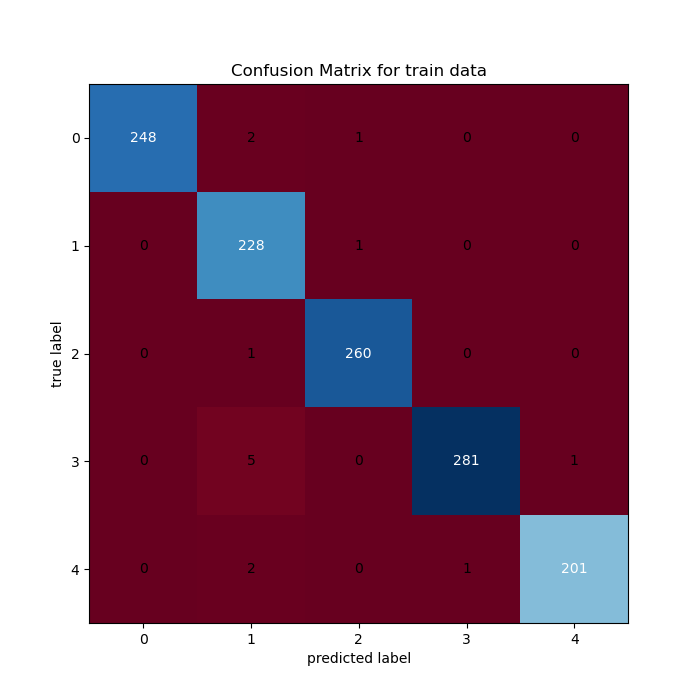
\includegraphics[height=2.5in]{Dataset_2a/dataset_2a_cmatrix_train_data_svc.png}
        \caption{Confusion Matrix for training data}
    \end{subfigure}%
    ~ 
    \begin{subfigure}[t]{0.5\textwidth}
        \centering
        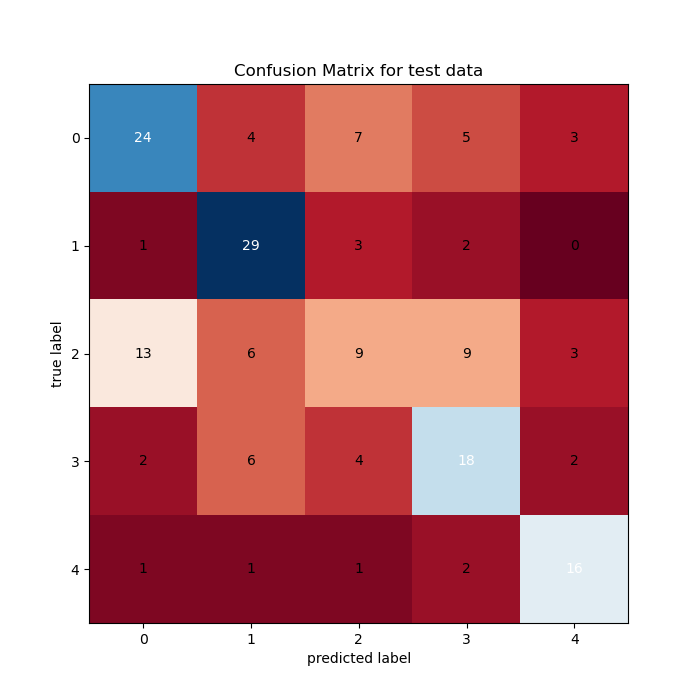
\includegraphics[height=2.5in]{Dataset_2a/dataset_2a_cmatrix_test_data_svc.png}
        \caption{Confusion Matrix for test data}
    \end{subfigure}%
    ~
    \caption{Confusion Matrix for the best model}
    \label{fig:13}
\end{figure}

%---------------------------------------------------------

\end{document}











